\documentclass[11pt]{article}
\usepackage[letterpaper,margin=0.9in]{geometry}
\usepackage{amsmath,amssymb,amsthm,lmodern,microtype}
\usepackage[T1]{fontenc}
\usepackage{xcolor,framed,booktabs,array,tikz}
\usetikzlibrary{arrows.meta,positioning,calc}
\usepackage[colorlinks=true,linkcolor=blue!60!black,urlcolor=blue!60!black]{hyperref}
\definecolor{shadecolor}{RGB}{240,244,250}
\definecolor{warncolor}{RGB}{253,242,235}
\definecolor{inkblue}{RGB}{28,76,122}
\definecolor{teal}{RGB}{0,117,116}
\newenvironment{keyidea}{\begin{shaded}\noindent\textbf{Key idea.} }{\end{shaded}}
\newenvironment{pitfall}{\begingroup\colorlet{shadecolor}{warncolor}\begin{shaded}\noindent\textbf{Common pitfall.} }{\end{shaded}\endgroup}
\newenvironment{recipe}{\begin{framed}\noindent\textbf{Recipe.} }{\end{framed}}
\newcommand{\R}{\mathbb R}
\newcommand{\T}{^{\mathsf T}}
\newcommand{\ones}{\mathbf 1}
\newcommand{\conv}{\operatorname{conv}}
\newcommand{\supp}{\operatorname{supp}}
\newcommand{\norm}[1]{\left\lVert#1\right\rVert}
\newtheorem{exercise}{Self-test}
\setlength{\parindent}{0pt}
\setlength{\parskip}{0.45em}
\setcounter{tocdepth}{1}
\hypersetup{pdftitle={Duality in Action - Homework 4 Study Guide},pdfauthor={Optimization companion notes}}
\begin{document}
\begin{center}
{\LARGE\bfseries Duality in Action}\\[8pt]
{\Large Stationary Distributions, Piecewise-Linear\\[3pt]
Optimization, and Robust Linear Programs}\\[10pt]
{\large A study guide for Homework 4}\\[5pt]
Optimization --- companion notes \quad | \quad September 27, 2026
\end{center}
\tableofcontents
\medskip
\begin{keyidea}
Homework 1 supplied the geometry: convex sets, convex combinations,
epigraphs, and separating hyperplanes. Homework 3 supplied certificates:
duality, complementary slackness, and theorems of the alternative.
Homework 4 uses these tools to prove existence, minimize a maximum,
and replace infinitely many requirements by a finite LP.
\end{keyidea}
\textbf{How to use this guide.} Read Sections 1--2, work the problems with
the separate solutions closed, and then use the relevant application
section to check your reasoning. Finish with the self-tests and the
one-page reference sheet. Optional Problem 5 is included as an extension.

{\small\textbf{Source:} supplied \texttt{hw04.pdf}, pp.\ 1--3. These companion
notes contain original explanations and examples, not an official solution
key. Numerical checks illustrate the theory; they do not replace proofs.\par}

\newpage
\section{The duality toolkit: from geometry to certificates}
Throughout, vector inequalities are componentwise. A variable without a
stated sign restriction is \emph{free}. Let $A\in\R^{m\times n}$.

\textbf{A feasible solution gives one bound; a dual solution gives the other.}
For the pair
\[
\min\{c\T x:Ax\ge b,\ x\ge0\},\qquad
\max\{b\T y:A\T y\le c,\ y\ge0\},
\]
feasibility gives $b\T y\le y\T Ax\le c\T x$. This is weak duality.
If these values agree, both solutions are optimal. For LPs, a feasible
problem with a finite optimal value attains that value, and its dual
has an optimizer with the same value: strong duality.

\begin{center}\renewcommand{\arraystretch}{1.35}
\begin{tabular}{@{}p{0.44\textwidth}p{0.48\textwidth}@{}}\toprule
\textbf{Fact} & \textbf{What it lets you do}\\\midrule
Weak duality & Certify a bound or optimality of a feasible pair.\\
Strong duality & Prove that some exact certificate exists.\\
Complementary slackness & Identify which constraints can carry nonzero weights.\\
Theorems of the alternative & Turn failure of feasibility into a separating certificate.\\\bottomrule
\end{tabular}
\end{center}

\textbf{Rebuild signs from the Lagrangian.} For a minimization problem
with inequalities $g_i(z)\le0$, use
$L(z,p)=f(z)+\sum_i p_i g_i(z)$ with $p_i\ge0$.
For feasible $z$, $L(z,p)\le f(z)$, so $\inf_zL$ is a lower bound.
A free variable with a nonzero linear coefficient makes that infimum
$-\infty$; its coefficient must vanish.

\textbf{Three pairs used repeatedly in this assignment:}
\[
\begin{array}{rcl}
\max\{q\T z:Bz=h,\ z\ge0\}
&\longleftrightarrow&\min\{h\T y:B\T y\ge q,\ y\text{ free}\},\\[5pt]
\max\{q\T z:Bz\le h,\ z\ge0\}
&\longleftrightarrow&\min\{h\T y:B\T y\ge q,\ y\ge0\},\\[5pt]
\min\{t:Ax-t\ones\le b\}
&\longleftrightarrow&\max\{-b\T p:A\T p=0,\ \ones\T p=1,\ p\ge0\}.
\end{array}
\]
Both $x$ and $t$ are free in the last pair.

\begin{pitfall}
Dual infeasibility alone does not imply primal unboundedness: the primal
might itself be infeasible. In Problem 1, explicitly checking primal
feasibility at $\lambda=0$ is what makes the argument work.
\end{pitfall}

\textbf{The recurring pattern.} Write a family of inequalities, combine
them with nonnegative weights, and make the unwanted variable disappear.
The remaining expression is a certificate that can be checked directly.

\newpage
\section{Stochastic matrices: existence from duality (Problem 1)}
A row-stochastic matrix satisfies $p_{ij}\ge0$ and
$\sum_jp_{ij}=1$. Think of $p_{ij}$ as the probability of moving from
state $i$ to state $j$. If the current distribution is a \emph{column}
$\pi$, the next distribution is $P\T\pi$.

An invariant distribution is a fixed point of this update:
\[
P\T\pi=\pi,\qquad \pi\ge0,\qquad\ones\T\pi=1.
\]
First find a nonzero nonnegative invariant vector, then normalize it.
This removes the normalization constraint while proving existence.

\begin{recipe}
\textbf{Turn existence into boundedness, and then contradict the dual.}
\begin{enumerate}
\item Form $\max\ones\T\lambda$ subject to
$(P\T-I)\lambda=0$, $\lambda\ge0$. The zero vector is feasible.
\item If no nonzero feasible vector exists, the optimal value is $0$.
\item Its dual is $\min0$ subject to $(P-I)y\ge\ones$, with $y$ free.
Strong duality would require a feasible dual solution.
\item Choose $k$ with $y_k=\max_jy_j$. Then
$(Py)_k=\sum_jp_{kj}y_j\le y_k$, so the $k$th dual inequality is impossible.
\end{enumerate}
Therefore a nonzero $\lambda\ge0$ exists, and
$\pi=\lambda/(\ones\T\lambda)$ is an invariant probability distribution.
\end{recipe}

\textbf{Why the maximum-coordinate trick works.} Each row of $P$ forms
a convex combination of the entries of $y$. A weighted average cannot
exceed the largest entry. Consequently, $P$ cannot increase \emph{every}
coordinate of any vector by at least $1$.

\begin{keyidea}
This connects Homework 1's convex-combination inequality to Homework 3's
duality. Geometry rules out a dual certificate; strong duality then forces
the invariant vector to exist.
\end{keyidea}

\textbf{Equivalent theorem-of-the-alternative view.} For a matrix $M$,
Gordan's alternative says exactly one of the following is possible:
\[
\exists y:\ My>0,
\qquad\text{or}\qquad
\exists\lambda\ge0,\ \lambda\ne0:\ M\T\lambda=0.
\]
With $M=P-I$, the maximum-coordinate argument rules out the first case.
The LP proof above supplies the same conclusion using ordinary LP duality.

\begin{pitfall}
$P\ones=\ones$ proves the existence of a \emph{right} eigenvector.
It does not by itself provide the nonnegative \emph{left} eigenvector
needed for $P\T\pi=\pi$. Keep the transpose and probability convention visible.
\end{pitfall}

\newpage
\section{Markov-chain intuition and what existence does not prove}
Consider the two-state chain
\[
P=\begin{pmatrix}0.9&0.1\\0.4&0.6\end{pmatrix}.
\]
\begin{center}
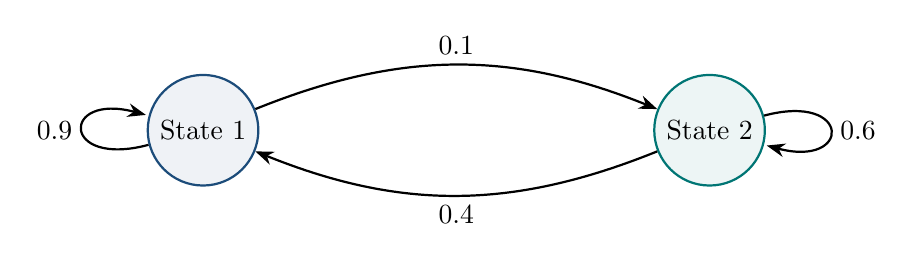
\begin{tikzpicture}[>=Stealth,thick,node distance=5cm]
\node[circle,draw=inkblue,fill=inkblue!7,minimum size=1.3cm] (a) {State 1};
\node[circle,draw=teal,fill=teal!7,minimum size=1.3cm,right=of a] (b) {State 2};
\draw[->,bend left=22] (a) to node[above] {$0.1$} (b);
\draw[->,bend left=22] (b) to node[below] {$0.4$} (a);
\draw[->] (a) edge[loop left] node[left] {$0.9$} (a);
\draw[->] (b) edge[loop right] node[right] {$0.6$} (b);
\end{tikzpicture}
\end{center}
At stationarity, net probability flow between the states balances:
$0.1\pi_1=0.4\pi_2$. Together with $\pi_1+\pi_2=1$, this gives
\[
\pi=(0.8,0.2)\T,\qquad
P\T\pi=(0.9\cdot0.8+0.4\cdot0.2,\;
0.1\cdot0.8+0.6\cdot0.2)\T=\pi.
\]
Pairwise flow balance is useful here because there are only two states;
it is not a required property of every stationary distribution in a
larger chain. Stationarity requires total inflow to equal total outflow
at each state.

\textbf{Connection to convex feasibility.} The probability simplex is
$\Delta_n=\{\pi\ge0:\ones\T\pi=1\}$.
The stationary distributions form
\[
\Delta_n\cap\ker(P\T-I),
\]
a convex polytope. If $\pi$ and $\rho$ are stationary, every mixture
$\theta\pi+(1-\theta)\rho$ is stationary too. The theorem says this
intersection is nonempty.

\textbf{Existence, uniqueness, and convergence are different claims.}
\begin{itemize}
\item \textbf{Existence always holds} for a finite row-stochastic matrix.
\item \textbf{Uniqueness can fail.} If $P=I$, every probability vector is stationary.
\item \textbf{Convergence can fail even with uniqueness.} If
$P=\left(\begin{smallmatrix}0&1\\1&0\end{smallmatrix}\right)$,
the unique stationary distribution is $(1/2,1/2)$, but a chain started
at $(1,0)$ alternates between $(1,0)$ and $(0,1)$.
\end{itemize}
As a later connection, finite irreducible chains have a unique stationary
distribution; adding aperiodicity gives convergence from every initial
distribution. These are stronger results than the homework asks you to prove.

\textbf{Connection to reinforcement learning.} Under a fixed stationary
policy, a finite-state environment induces a transition matrix. An invariant
distribution describes a probability flow that remains unchanged under
that policy. Whether the distribution from an arbitrary initial state
converges to it needs the additional assumptions above.

\newpage
\section{Minimizing a maximum: the epigraph LP (Problem 2)}
Let $f(x)=\max_i(a_i\T x-b_i)$, with rows $a_i\T$ collected in $A$.
Each affine piece is convex; a pointwise maximum of convex functions
is convex. It may be nondifferentiable where several pieces meet.

\textbf{The epigraph is a polyhedron.} A scalar $t$ is above the maximum
exactly when it is above every piece:
\[
t\ge f(x)\ \Longleftrightarrow\ a_i\T x-b_i\le t\quad\forall i.
\]
Hence
\[
\min_xf(x)=\min_{x,t}\{t:Ax-t\ones\le b\},\qquad x,t\text{ free}.
\]
This is Homework 1's epigraph idea used as a modeling tool.

\textbf{Derive the dual, rather than memorize it.}
For $p\ge0$,
\[
L(x,t,p)=t+p\T(Ax-t\ones-b)
=(A\T p)\T x+(1-\ones\T p)t-b\T p.
\]
To avoid $\inf_{x,t}L=-\infty$, both free-variable coefficients must vanish:
\[
\boxed{A\T p=0,\qquad\ones\T p=1,\qquad p\ge0.}
\]
The remaining constant is $-b\T p$. Thus these weights give the dual
$\max -b\T p$ under the displayed constraints.

\textbf{What each constraint means:}
\begin{itemize}
\item $p\ge0$: combine valid inequalities without reversing them.
\item $\ones\T p=1$: a convex combination cannot exceed the largest piece.
\item $A\T p=0$: balance the slopes so the lower bound does not depend on $x$.
\end{itemize}
Indeed, for every feasible $p$ and every $x$,
\[
f(x)\ge\sum_i p_i(a_i\T x-b_i)=-b\T p.
\]
The epigraph LP is feasible. Under the assumed finite value, LP attainment
and strong duality show that the best such lower bound equals the minimum.

\begin{pitfall}
Do not add $t\ge0$. The maximum of affine functions can have a negative
minimum. Likewise, adding $x\ge0$ changes the homework and changes the
dual condition $A\T p=0$ to an inequality.
\end{pitfall}

\textbf{A useful modeling extension.} Chebyshev fitting,
$\min_x\norm{Cx-d}_\infty$, is also an LP: minimize $t$ subject to
$-t\ones\le Cx-d\le t\ones$. It is the maximum of the affine residuals
and their negatives, so the same epigraph method applies.

\newpage
\section{Active slopes, subgradients, and a worked example}
Take
\[
f(x)=\max\{2x,\,-x+3,\,x-1\}.
\]
The first two pieces meet at $x^*=1$, with $f(1)=2$; the third has value $0$.
\begin{center}
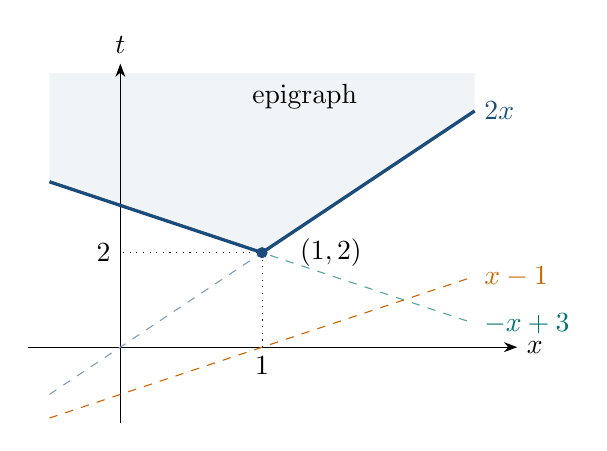
\begin{tikzpicture}[x=1.8cm,y=0.60cm,>=Stealth]
\fill[inkblue!6] (-.5,3.5)--(1,2)--(2.5,5)--(2.5,5.8)--(-.5,5.8)--cycle;
\draw[->] (-.65,0)--(2.8,0) node[right] {$x$};
\draw[->] (0,-1.6)--(0,6.0) node[above] {$t$};
\draw[inkblue!55,dashed] (-.5,-1)--(2.5,5);
\draw[teal!65,dashed] (-.5,3.5)--(2.5,.5);
\draw[orange!80!black,dashed] (-.5,-1.5)--(2.5,1.5);
\draw[very thick,inkblue] (-.5,3.5)--(1,2)--(2.5,5);
\draw[dotted] (1,0) node[below] {$1$}--(1,2)--(0,2) node[left] {$2$};
\fill[inkblue] (1,2) circle (2pt);
\node[anchor=west] at (1.2,2.0) {$(1,2)$};
\node[inkblue,anchor=west] at (2.5,5) {$2x$};
\node[teal,anchor=west] at (2.5,.5) {$-x+3$};
\node[orange!80!black,anchor=west] at (2.5,1.5) {$x-1$};
\node at (1.3,5.3) {epigraph};
\end{tikzpicture}
\end{center}
Choose $p=(1/3,2/3,0)$. Its entries sum to $1$, and
$2p_1-p_2+p_3=0$. Since $b=(0,-3,1)$, the dual lower bound is
$-b\T p=2$. The candidate attains this bound, proving optimality.

\textbf{Why only active slopes matter.} At an optimal pair, complementary
slackness says
\[
p_i^*\big[t^*-(a_i\T x^*-b_i)\big]=0.
\]
An inactive piece has positive slack and therefore zero weight.
If $I(x)=\{i:a_i\T x-b_i=f(x)\}$, optimality is equivalent to
\[
\boxed{0\in\conv\{a_i:i\in I(x)\}.}
\]
In the example, $0=(1/3)\cdot2+(2/3)\cdot(-1)$.

\textbf{Connection to subgradients.} A subgradient $g$ at $x$ satisfies
$f(z)\ge f(x)+g\T(z-x)$ for all $z$. For a finite maximum of affine
functions, $\partial f(x)=\conv\{a_i:i\in I(x)\}$.
Thus $0\in\partial f(x)$ is the nonsmooth analogue of $\nabla f(x)=0$.
This previews first-order optimization methods.

\textbf{Connection to minimax.} Since a maximum equals the maximum over
probability weights, $f(x)=\max_{p\in\Delta_m}p\T(Ax-b)$.
Strong LP duality gives $\inf_x\max_{p\in\Delta_m}p\T(Ax-b)
=\max_{p\in\Delta_m}\inf_x p\T(Ax-b)$ when the value is finite.
The opponent's optimal mixture cancels all dependence on $x$.

\newpage
\section{Symmetry and certificates of optimality (Problem 3)}
Consider
\[
\min\{c\T x:Ax\ge c,\ x\ge0\},\qquad A=A\T.
\]
If $Ax^*=c$ and $x^*\ge0$, the same vector works on both sides of the
primal--dual pair:
\[
\text{dual:}\quad\max\{c\T y:A\T y\le c,\ y\ge0\},\qquad y^*=x^*.
\]
It is feasible because $A\T x^*=Ax^*=c$, and the objectives agree.
Weak duality proves optimality immediately.

\textbf{Read the proof as a weighted sum of constraints.} For any feasible $x$,
\[
\underbrace{c\T x}_{\text{candidate cost}}
=(Ax^*)\T x
=(x^*)\T Ax
\ge(x^*)\T c
=\underbrace{c\T x^*}_{\text{certified lower bound}}.
\]
The nonnegative entries of $x^*$ are precisely the weights applied to
$Ax\ge c$. Symmetry makes their weighted left side equal the objective.

\begin{keyidea}
Symmetry is used to move $A$ across the inner product. Positive
semidefiniteness is not needed: the objective and constraints are linear,
so the problem is an LP regardless of the eigenvalues of $A$.
\end{keyidea}

\textbf{An indefinite example.}
Let $A=\left(\begin{smallmatrix}0&1\\1&0\end{smallmatrix}\right)$ and
$c=(1,1)$. Its eigenvalues are $1$ and $-1$, but $x^*=(1,1)$ is feasible
with $Ax^*=c$. The constraints are $x_2\ge1$, $x_1\ge1$, so the minimum
of $x_1+x_2$ is $2$.

\textbf{Why symmetry matters.}
Take $A=\left(\begin{smallmatrix}1&1\\0&1\end{smallmatrix}\right)$,
$c=(2,1)$, and $x^*=(1,1)$. Although $Ax^*=c$ and $x^*\ge0$,
its cost is $3$. The feasible point $(0,2)$ costs $2$.
The proposed certificate fails because $A\T x^*=(1,2)\nleq(2,1)$.

\textbf{Connection to complementary slackness and KKT.}
For a general feasible pair $(x,y)$ in this LP, the gap decomposes as
\[
c\T x-c\T y
=x\T(c-A\T y)+y\T(Ax-c)\ge0.
\]
At the special pair $x=y=x^*$, both slack vectors vanish. This is the
linear-programming version of the KKT optimality conditions: feasibility,
dual feasibility, stationarity, and complementary slackness.

\begin{pitfall}
Tight primal constraints alone do not prove optimality. You must also
produce a valid bound, such as a dual-feasible vector with matching cost.
Nor does this argument claim the optimizer is unique.
\end{pitfall}

\newpage
\section{Robust right-hand sides and the order of quantifiers (Problem 4)}
A robust constraint must hold for \emph{every} allowed uncertainty value.
The decision $x$ is chosen once, before the uncertainty is revealed.
For a nonempty uncertainty set $\mathcal U$,
\[
Ax\ge b\ \forall b\in\mathcal U
\ \Longleftrightarrow\
(Ax)_i\ge\sup_{b\in\mathcal U}b_i\quad\forall i.
\]
For $Ax\le b$, use the coordinatewise \emph{infimum} instead.

In Problem 4, the displayed set is
$\mathcal U=\{b\ge0:\ones\T b\le1\}$; the extra $b_i\le1$ bounds
are redundant. It is a simplex, despite being called a unit box.
Each $e_i\in\mathcal U$, so each coordinate can individually reach $1$.
The exact counterpart is therefore $Ax\ge\ones$.

\begin{center}
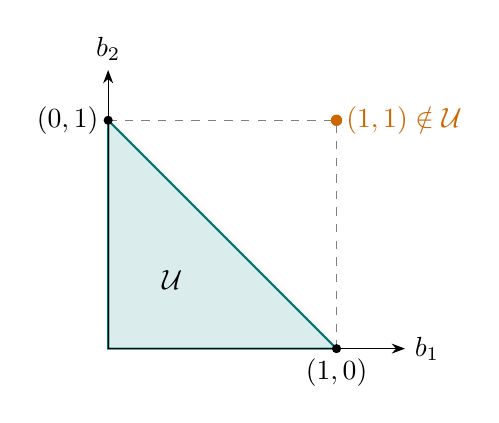
\begin{tikzpicture}[scale=2.9,>=Stealth]
\fill[teal!14] (0,0)--(1,0)--(0,1)--cycle;
\draw[thick,teal] (0,0)--(1,0)--(0,1)--cycle;
\draw[->] (0,0)--(1.3,0) node[right] {$b_1$};
\draw[->] (0,0)--(0,1.22) node[above] {$b_2$};
\draw[dashed,gray] (1,0)--(1,1)--(0,1);
\fill (1,0) circle(.02) node[below] {$(1,0)$};
\fill (0,1) circle(.02) node[left] {$(0,1)$};
\fill[orange!80!black] (1,1) circle(.025) node[right] {$(1,1)\notin\mathcal U$};
\node at (.28,.3) {$\mathcal U$};
\end{tikzpicture}
\end{center}
For two rows, scenario $(1,0)$ forces the first threshold to $1$, while
$(0,1)$ forces the second threshold to $1$. The two worst cases need not
occur in the same scenario. Universal quantifiers commute:
$\forall b\,\forall i$ is the same as $\forall i\,\forall b$.

\begin{pitfall}
Do not replace the vector constraint by
$\sum_i(Ax)_i\ge\max_{b\in\mathcal U}\sum_i b_i=1$.
That is weaker: $(Ax)=(1,0)$ passes the sum test but fails against
$b=(0,1)$. Row-by-row guarantees are essential.
\end{pitfall}

\textbf{Why the uncertainty budget disappears here.} With
$\mathcal U_\Gamma=\{0\le b\le\ones:\ones\T b\le\Gamma\}$,
$\Gamma\ge0$, the answer is $Ax\ge\min\{1,\Gamma\}\ones$.
Once $\Gamma\ge1$, each coordinate can already hit its individual maximum.
In a \emph{single} constraint containing a sum of uncertain terms, the
budget can still matter substantially.

\newpage
\section{Uncertain coefficients: support functions and dual LPs}
For coefficient uncertainty, the uncertain vector multiplies the decision:
\[
a\T x\le\beta\quad\forall a\in\mathcal U
\quad\Longleftrightarrow\quad
\sigma_{\mathcal U}(x):=\sup_{a\in\mathcal U}a\T x\le\beta.
\]
$\sigma_{\mathcal U}$ is the \emph{support function}. It is convex because
it is a pointwise supremum of linear functions of $x$; it may equal
$+\infty$ for an unbounded set. This directly connects robustness to
Homework 1's convex-function calculus.

\textbf{Equality constraints and nonnegative uncertain coefficients.}
For nonempty $\mathcal U_2=\{a:D_2a=d_2,\ a\ge0\}$, dualize the
adversary's maximization with $x$ held fixed:
\[
\sup_{a\ge0,\ D_2a=d_2}x\T a
\quad\longleftrightarrow\quad
\inf_{y_2\text{ free},\ D_2\T y_2\ge x}d_2\T y_2.
\]
The exact robust counterpart is the \emph{existence} of a certificate:
\[
\boxed{\exists y_2\text{ free}:\quad D_2\T y_2\ge x,\quad d_2\T y_2\le\beta.}
\]
Weak duality proves sufficiency: for every allowed $a$,
$x\T a\le y_2\T D_2a=y_2\T d_2\le\beta$.
If robustness holds, the nonempty inner LP has finite value, so strong
duality supplies a certificate and proves necessity.

\textbf{Inequality constraints and nonpositive uncertain coefficients.}
For $\mathcal U_3=\{a:D_3a\ge d_3,\ a\le0\}$, first use $z=-a$:
\[
\sup_{z\ge0,\ D_3z\le-d_3}(-x)\T z
\quad\longleftrightarrow\quad
\inf_{\mu_3\ge0,\ D_3\T\mu_3\ge-x}(-d_3)\T\mu_3.
\]
Thus, for nonempty $\mathcal U_3$,
\[
\boxed{\exists\mu_3\ge0:\quad D_3\T\mu_3\ge-x,\quad-d_3\T\mu_3\le\beta.}
\]

\begin{recipe}
\textbf{Convert a robust coefficient constraint to finite constraints.}
\begin{enumerate}
\item Freeze $x$ and maximize the uncertain left-hand side over its set.
\item Normalize signs, such as $z=-a\ge0$, before forming the dual.
\item Introduce the dual variables as extra decision variables.
\item Require dual feasibility and a dual objective no larger than the RHS.
\item Justify exactness using nonemptiness, bounded value, and strong duality.
\end{enumerate}
\end{recipe}
The new variables are certificates of robustness, not extra uncertain
quantities. No additional sign restriction on $x$ is implied.

\newpage
\section{The optional problem, edge cases, and broader connections}
\textbf{Resolve the handout's notation.} For $A\in\R^{m\times n}$ and
$x\in\R^n$, use $Ax\le b$ for the first block of Problem 5.
The printed $A\T x$ needs $A\in\R^{n\times m}$ instead. The final set
is $\mathcal U_3$, correcting the repeated $\mathcal U_2$ label.

For a nonempty polytope $\mathcal U_1$, precompute
$\underline b_i=\min_{b\in\mathcal U_1}b_i$. With all sets nonempty,
the finite LP is
\[
\begin{aligned}
\min_{x,y_2,\mu_3}\quad &c\T x\\
\text{s.t.}\quad&Ax\le\underline b,\\
&D_2\T y_2\ge x,\qquad d_2\T y_2\le b_2,\\
&D_3\T\mu_3\ge-x,\qquad-d_3\T\mu_3\le b_3,\\
&\mu_3\ge0,\qquad x,y_2\text{ free}.
\end{aligned}
\]
If $D_j$ has $r_j$ rows, its certificate vector has $r_j$ entries.
The problem uses $n+r_2+r_3$ variables. The coordinatewise minima need
not all occur at the same $b\in\mathcal U_1$.

\textbf{Two small sets that make the formulas tangible.}
\begin{enumerate}
\item If $\mathcal U_2=\{a\ge0:a_1+a_2=1\}$, its support function is
$\max(x_1,x_2)$. The dual certificate is a scalar $y$ satisfying
$y\ge x_1,x_2$ and $y\le\beta$.
\item If $\mathcal U_3=\{a\le0:a_1+a_2\ge-1\}$, its vertices are
$0,-e_1,-e_2$. Its support is $\max(0,-x_1,-x_2)$.
The robust constraint is $\beta\ge0$ and $x_1,x_2\ge-\beta$.
\end{enumerate}

\textbf{Empty sets.} A universal statement over an empty set is true.
Check emptiness by LP feasibility, then omit the associated constraint
block if its uncertainty set is empty.

\textbf{Unbounded sets.} With $\mathcal U=\{a\ge0:a_1=1\}$,
$\sigma_{\mathcal U}(x)=x_1$ if $x_2\le0$ and $+\infty$ if $x_2>0$.
The dual automatically enforces $x_2\le0$. An unbounded uncertainty
set can therefore still permit robust decisions.

\textbf{Beyond polytopes: uncertainty geometry chooses the model.}
For $a=a_0+u$ with $\norm{u}_2\le\rho$, Cauchy--Schwarz gives
$\sup a\T x=a_0\T x+\rho\norm{x}_2$. Robustness becomes a second-order
cone constraint. For $\norm{u}_\infty\le\rho$, the answer is
$a_0\T x+\rho\norm{x}_1$, which can be modeled by an LP with absolute-value
auxiliaries. These are consequences of the uncertainty set's support function.

\newpage
\section{Self-tests: work these before opening the answers}
\begin{exercise}
Let $P=\left(\begin{smallmatrix}3/4&1/4\\1/2&1/2\end{smallmatrix}\right)$.
Find its stationary distribution and verify it by multiplication.
\end{exercise}
\begin{exercise}
For $P=I$, how many stationary distributions exist? For the two-state
swap matrix, does a unique stationary distribution imply convergence
from $(1,0)$? Explain the distinction in one sentence.
\end{exercise}
\begin{exercise}
Write the epigraph LP and its dual for
$\min_x\max\{x+1,-2x+4\}$. Find a primal optimum and dual certificate.
\end{exercise}
\begin{exercise}
For $f(x)=\max\{x,2x\}$, both pieces are active at $x=0$.
Is $0$ a minimizer? What does the convex hull of the active slopes say?
\end{exercise}
\begin{exercise}
For a finite maximum of affine functions on all of $\R^n$, show that
the value is finite if and only if $0\in\conv\{a_1,\ldots,a_m\}$.
Hint: use a feasible dual mixture in one direction and strict separation
from a compact convex hull in the other.
\end{exercise}
\begin{exercise}
Let $A=\left(\begin{smallmatrix}0&1\\1&0\end{smallmatrix}\right)$,
$c=(2,3)$. Find $x^*\ge0$ with $Ax^*=c$ and certify the minimum of
$c\T x$ over $Ax\ge c$, $x\ge0$.
\end{exercise}
\begin{exercise}
Let $\mathcal U=\{b\ge0:b_1+b_2\le1\}$. Give the exact counterparts
of (i) $Ax\ge b$ for all $b\in\mathcal U$ and (ii) $Ax\le b$ for all
$b\in\mathcal U$. Explain why the two answers differ.
\end{exercise}
\begin{exercise}
If $\mathcal U=\{a\ge0:a_1+a_2=1\}$, eliminate uncertainty from
$a\T x\le5$. Derive the same result through a scalar dual variable.
\end{exercise}
\begin{exercise}
If $\mathcal U=\{a\le0:a_1+a_2\ge-1\}$, eliminate uncertainty from
$a\T x\le\beta$. Can any $x$ work if $\beta=-1$?
\end{exercise}
\begin{exercise}
If $\mathcal U=\{a\ge0:a_1=1\}$, when does $a\T x\le3$ hold for all
$a\in\mathcal U$? What changes if the uncertainty set is empty?
\end{exercise}
\begin{exercise}
Suppose $a=a_0+u$, $\norm{u}_2\le2$. Write the exact counterpart of
$a\T x\le7$. Which Homework 1 inequality proves it?
\end{exercise}

\newpage
\section{Self-test answers and proof sketches}
\begin{enumerate}
\item Flow balance gives $\frac14\pi_1=\frac12\pi_2$, so
$\pi=(2/3,1/3)$. Directly,
$P\T\pi=(\frac34\frac23+\frac12\frac13,\frac14\frac23+\frac12\frac13)
=(2/3,1/3)$.
\item Every probability vector is stationary for $I$. The swap matrix
has the unique stationary vector $(1/2,1/2)$, yet the stated initial
distribution alternates. A fixed point can exist uniquely without all
iterates converging to it.
\item Epigraph: $\min t$ subject to $x+1\le t$, $-2x+4\le t$, with
$x,t$ free. Dual: $\max p_1+4p_2$ subject to
$p_1-2p_2=0$, $p_1+p_2=1$, $p\ge0$. The intersection gives
$x^*=1,t^*=2$; $p=(2/3,1/3)$ gives the matching value $2$.
\item No. The active slopes are $1,2$, whose convex hull $[1,2]$
excludes zero. In fact, for $x<0$, $f(x)=x$, so the problem is
unbounded below. Ties alone do not prove optimality.
\item If $0=\sum_i p_i a_i$ with $p\in\Delta_m$, then
$f(x)\ge-\sum_i p_i b_i$ for every $x$, and $f(0)$ is finite.
Conversely, if the compact convex hull excludes $0$, strict separation
gives a direction $d$ and $\epsilon>0$ with $a_i\T d\le-\epsilon$
for every $i$. Then $f(td)\le-t\epsilon+\max_i(-b_i)\to-\infty$.
\item $x^*=(3,2)$, with cost $2\cdot3+3\cdot2=12$.
Symmetry makes $y=x^*$ dual feasible, and its value is also $12$.
The matrix is indefinite; that is irrelevant to this LP certificate.
\item (i) $Ax\ge(1,1)\T$; each coordinate can reach $1$.
(ii) $Ax\le(0,0)\T$; $b=0$ is allowed and is the smallest RHS
componentwise. A $\ge$ constraint fears a larger RHS, while a $\le$
constraint fears a smaller one.
\item The counterpart is $x_1\le5$, $x_2\le5$.
The scalar dual satisfies $y\ge x_1$, $y\ge x_2$, $y\le5$;
such $y$ exists exactly under those two inequalities.
\item The support is $\max(0,-x_1,-x_2)$. Thus
$\beta\ge0$ and $x_1,x_2\ge-\beta$. For $\beta=-1$, no $x$ works
because $a=0$ is allowed and would require $0\le-1$.
\item Precisely $x_1\le3$ and $x_2\le0$. If $x_2>0$, the adversary
can send $a_2$ to infinity. If the set is empty, the universal
constraint is vacuous and imposes no restriction on $x$.
\item $a_0\T x+2\norm{x}_2\le7$. Cauchy--Schwarz bounds
$u\T x\le2\norm{x}_2$, with equality at
$u=2x/\norm{x}_2$ for $x\ne0$; $x=0$ is immediate.
\end{enumerate}
\begin{keyidea}
When a proof feels abstract, ask what the certificate is and how to check
it: an invariant vector, a balancing probability mixture, a matching dual
solution, or a finite set of multipliers bounding every uncertainty scenario.
\end{keyidea}

\newpage
\section{One-page reference sheet}
\small
\textbf{Duality.} Feasible primal + feasible dual + equal objectives
$\Rightarrow$ both optimal. A feasible LP with finite value has an
attained optimum and an equal attained dual optimum. Dual infeasibility
requires a primal-feasibility check before concluding unboundedness.

\textbf{Stochastic matrices.}
$P\ge0$, $P\ones=\ones$. A probability column evolves as
$\pi_{k+1}=P\T\pi_k$. Stationarity:
$P\T\pi=\pi$, $\pi\ge0$, $\ones\T\pi=1$.
\[
\max_{\lambda\ge0}\{\ones\T\lambda:(P\T-I)\lambda=0\}
\ \longleftrightarrow\
\min_y\{0:(P-I)y\ge\ones\}.
\]
The dual fails at a largest coordinate of $y$, forcing a nonzero primal
vector. Normalize it. Existence $\ne$ uniqueness $\ne$ convergence.

\textbf{Maximum of affine functions.}
\[
\min_x\max_i(a_i\T x-b_i)
=\min_{x,t}\{t:Ax-t\ones\le b\}
=\max_{p\ge0}\{-b\T p:A\T p=0,\ \ones\T p=1\},
\]
with finite value assumed and $x,t$ free. Lower bound:
$\max_i(a_i\T x-b_i)\ge\sum_i p_i(a_i\T x-b_i)=-b\T p$.
Optimal weights live on active pieces. Optimality at $x$:
$0\in\conv\{a_i:i\in I(x)\}=\partial f(x)$.
Finite value iff $0\in\conv\{a_1,\ldots,a_m\}$.

\textbf{Symmetry certificate.}
For $\min c\T x$ s.t.\ $Ax\ge c$, $x\ge0$, if
$A=A\T$, $Ax^*=c$, $x^*\ge0$, use dual $y=x^*$.
Directly: $c\T x=(x^*)\T Ax\ge(x^*)\T c$.

\textbf{Robust RHS.} For nonempty $\mathcal U$:
\[
Ax\ge b\ \forall b\in\mathcal U\iff (Ax)_i\ge\sup_{b\in\mathcal U}b_i;
\quad
Ax\le b\ \forall b\in\mathcal U\iff (Ax)_i\le\inf_{b\in\mathcal U}b_i.
\]
The extrema are coordinatewise; the assembled vector need not lie in
$\mathcal U$. For $\mathcal U=\{b\ge0:\ones\T b\le1\}$, the first
counterpart is $Ax\ge\ones$.

\textbf{Robust coefficients.} Replace $a\T x\le\beta$ for all
$a\in\mathcal U$ by $\sigma_{\mathcal U}(x)\le\beta$.
For the nonempty sets below, exact finite certificates are:
\[
\begin{array}{ll}
\mathcal U=\{a:D a=d,\ a\ge0\}:&
\exists y\text{ free}:\ D\T y\ge x,\ d\T y\le\beta;\\[4pt]
\mathcal U=\{a:D a\ge d,\ a\le0\}:&
\exists\mu\ge0:\ D\T\mu\ge-x,\ -d\T\mu\le\beta.
\end{array}
\]
Empty uncertainty $\Rightarrow$ omit its block. Unbounded support value
$\Rightarrow$ that decision fails robustness. Unbounded set alone is
not enough to conclude failure.

\textbf{Final checks.} Dimensions; free versus signed variables; min
versus max; $\le$ versus $\ge$; nonempty uncertainty; exactness via strong
duality; candidate feasibility; matching objective values.

\vfill
\footnotesize\textit{Companions:} \texttt{hw04\_solutions.pdf} contains full worked proofs.\\
\texttt{verify.py} checks examples; \texttt{verification\_results.json} records the results.
\end{document}
